\documentclass[aspectratio=169]{beamer}
\usepackage[english,russian]{babel}
\usepackage{tikz}
\usetikzlibrary{shapes.geometric}
\usetikzlibrary{arrows}
\usepackage{amsmath,amssymb}
\usepackage{array}
\usepackage{graphbox}
\usepackage{xcolor}

\newcommand{\yicon}{
\includegraphics[width=20px]{icon-check.png}}
\newcommand{\nicon}{
\includegraphics[width=20px]{icon-cross.png}}

\setbeamertemplate{footline}[frame number]
\setbeamertemplate{navigation symbols}{}

\setbeamercolor{palette primary}{fg=black,bg=white}
\setbeamercolor{palette secondary}{fg=black,bg=white}
\setbeamercolor{structure}{fg=black,bg=white}

% title frame
\defbeamertemplate*{title page}{mytheme}[1][]
{
  \begin{tikzpicture}[remember picture,overlay]
  \filldraw[white]
    (current page.north west) --
    (current page.north east) --
    ([xshift=0cm,yshift=-2cm]current page.north east)  --
    ([xshift=0cm,yshift=-2cm]current page.north west) -- cycle
    ;
  
  \node[opacity=0.1] at ([xshift=-2.5cm,yshift=-0.3cm]current page.north east) {
\includegraphics[width=12cm]{wcc}};
  
  \node[text=black,anchor=south west,font=\sffamily\LARGE,text width=.8\paperwidth] at ([xshift=-100pt,yshift=-1cm]current page.center)(title){\raggedright\inserttitle};
    
  \node[text=black,anchor=south west,font=\sffamily\small,text width=.6\paperwidth] at ([xshift=-100pt,yshift=-1.5cm]current page.center)(institute){\raggedright\insertinstitute};
   
  \node[text=black,font=\large\sffamily,anchor=south west] at ([xshift=30pt,yshift=0.5cm]current page.south west)(date){\insertdate};
  
  \node[text=black,font=\large\sffamily,anchor=south west] at ([yshift=5pt]date.north west)(author){\insertauthor};
  \end{tikzpicture}
}

% definition of the symbols used in itemize
\newcommand\mysymbol{%
  \begin{tikzpicture}[xscale=0.85]
\draw[black, thick]  circle (1.5 pt);             
  \end{tikzpicture}%
  }

% definition of the itemize templates
\defbeamertemplate*{itemize item}{mysymbol}{\small\raise0.5pt\hbox{\mysymbol}}
\defbeamertemplate*{itemize subitem}{mysymbol}{\footnotesize\raise0.5pt\hbox{\mysymbol}}
\defbeamertemplate*{itemize subsubitem}{mysymbol}{\footnotesize\raise0.5pt\hbox{\mysymbol}}

\title[Анонимность транзакций: прошлое, настоящее и будущее]{Анонимность транзакций: прошлое, \\ настоящее и будущее}
\author{Саранг Ноезер(Sarang Noether), кандидат наук}
\date{Хэллоуин 2019}

\institute{World Crypto Con, Лас-Вегас}

\begin{document}

\begin{frame}[plain]
\maketitle
\end{frame}


\begin{frame}
\frametitle{Отказ от ответственности}
\begin{columns}
\begin{column}{0.2\textwidth}

\includegraphics[width=0.9\textwidth]{icon-jack.png}
\end{column}
\begin{column}{0.8\textwidth}
Взгляды, представленные в данной презентации, принадлежат исключительно её автору и не обязательно отражают взгляды других людей, организаций или сообщества. \\~\\

Материал, представленный в презентации, носит образовательный характер и не должен рассматриваться в качестве финансовых, юридических или каких-либо других рекомендаций или поддержки какого бы то ни было рода. \\~\\

Автор является независимым исследователем, математиком, входящим в состав рабочей группы Исследовательской лаборатории Monero (Monero Research Lab) и получающим финансовую поддержку от сообщества Monero.
\end{column}
\end{columns}
\end{frame}


\begin{frame}{Цели}
Вы должны понимать и ценить:
\begin{itemize}
\item \textbf{важность} взаимозаменяемости и анонимности в рамках протоколов транзакций;
\item \textbf{развитие} используемых криптографических подходов;
\item \textbf{отличия} моделей транзакций и систем доказательства;
\item как \textbf{компромиссы} с точки зрения эффективности и доверия влияют на выбор технического решения. \\~\\
\end{itemize}

\begin{columns}
\begin{column}{0.2\textwidth}
\centering

\includegraphics[width=0.6\textwidth]{icon-ghost.png}
\end{column}
\begin{column}{0.6\textwidth}
\centering
Математика может напугать, поэтому здесь её не будет.
\end{column}
\begin{column}{0.2\textwidth}
\centering

\includegraphics[width=0.6\textwidth]{icon-ghost.png}
\end{column}
\end{columns}
\end{frame}


\begin{frame}{Взаимозаменяемость?}
Анонимность и взаимозаменяемость связаны. \textbf{Взаимозаменяемость} может означать неотличимость. Можно ли занести определённые средства в чёрный список? \\~\\

Прозрачные реестры, такие как у Bitcoin, совершенно не обеспечивают взаимозаменяемости и анонимности.
\begin{itemize}
\item Адреса отображаются в цепочке как часть транзакций
\item Суммы указываются в открытую.
\item Активы имеют отличную друг от друга историю и свойства.
\end{itemize}

{\Huge $$\begin{array}{l} 
\includegraphics[width=40pt]{btc.png} \end{array} \quad \neq \quad  \begin{array}{l} 
\includegraphics[width=40pt]{btc.png} \end{array}$$}
\end{frame}


\begin{frame}{Основные принципы построения транзакций}
Транзакции (в первую очередь) включают в себя \textbf{входы}, \textbf{выходы}, и \textbf{подтверждения}. \\~\\

Транзакция берёт входы, используя подтверждения, и генерирует новые выходы. Цифровая подпись является самым основным подтверждением. \\~\\

\begin{figure}
\begin{tikzpicture}[thick,square/.style={regular polygon,regular polygon sides=4}]
\node [square,draw] (auths) {Подтв.};
\node [rectangle,draw,left=60pt,above=40pt,at=(auths.west),fill=gray!30] (input1) {Вход};
\node [rectangle,draw,left=60pt,below=40pt,at=(auths.west),fill=gray!30] (input2) {Вход};
\node [circle,draw,above=10pt,at=(auths.north)] (sk1) {sk};
\node [circle,draw,below=10pt,at=(auths.south)] (sk2) {sk};
\node [rectangle,draw,right=60pt,at=(auths.east),fill=gray!30] (output2) {Выход};
\node [rectangle,draw,above=20pt,at=(output2.north),fill=gray!30] (output1) {Выход};
\node [rectangle,draw,below=20pt,at=(output2.south),fill=gray!30] (output3) {Выход};

\draw [->] (input1) -- (auths);
\draw [->] (input2) -- (auths);
\draw [dashed,-] (sk1) -- (input1);
\draw [dashed,-] (sk2) -- (input2);
\draw [dashed,->] (sk1) -- (auths);
\draw [dashed,->] (sk2) -- (auths);
\draw [->] (auths) -- (output1);
\draw [->] (auths) -- (output2);
\draw [->] (auths) -- (output3);
\end{tikzpicture}
\end{figure}

\end{frame}


\begin{frame}{Граф транзакции}
Любой участник сети может проанализировать прозрачный реестр и изучить поток средств в транзакциях. \\~\\

\begin{figure}
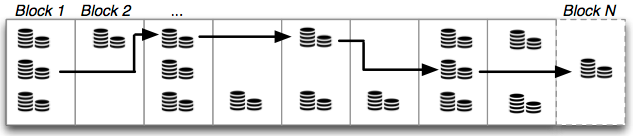
\includegraphics[width=0.7\textwidth]{btc-chain.png}
\end{figure}

Темой \underline{очень многих} исследований стали методы анализа блокчейна на основе его прозрачности.
\end{frame}


\begin{frame}{Стоит ли беспокоиться?}
Прозрачность и отсутствие взаимозаменяемости могут иметь последствия, которые вам могут как понравиться, так и не понравиться:

\begin{itemize}
\item \textbf{Цензурирование}: майнеры и другие лица могут цензурировать транзакции на основе информации адресов, суммы, местоположения и других данных/метаданных.
\item \textbf{Рынки}: определённые типы или объёмы активов могут принести персональную надбавку в зависимости от истории или способов использования.
\item \textbf{Связывание}: любая третья сторона, обладающая доступом к публичному блокчейну, может связать данные и суммы и попытаться привязать их к личности, что повышает персональный риск.
\item \textbf{Конкуренция}: к онкурирующие бизнесмены банально могут получить информацию о транзакциях, а значит, информацию частного характера или деловую информацию.
\item \textbf{Регулирование}: некоторые юрисдикции могут ввести правила, обязующие соблюдать анонимность финансовой информации при хранении и передаче. \\~\\
\end{itemize}

В случае с  ``анонимными монетами" has it reversed! Shouldn't all bathrooms have doors?
\end{frame}


\begin{frame}{Спектр общих подходов}
\begin{figure}
\centering
\begin{tikzpicture}[thick]
\node (mixers) {Прозрачные миксеры};
\node [below=40pt,at=(mixers.south)] (decoys) {Специфические средства обеспечения неопределённости};
\node [below=40pt,at=(decoys.south)] (acc) {Накопители};
\node [right=60pt,at=(decoys.east)] (mw) {Mimblewimble};

\draw [->] (mixers) -- (decoys);
\draw [->] (decoys) -- (acc);
\end{tikzpicture}
\end{figure}
\end{frame}


\begin{frame}{Пример: прозрачные миксеры}
\textbf{Прозрачные миксеры} берут прозрачные средства, возможно, принадлежащие различным владельцам, и включают их в одну транзакцию. Подтверждения могут быть изменены соответствующим образом, но, как правило, это не требует каких-либо новых математических решений.

\begin{figure}
\begin{tikzpicture}[thick,square/.style={regular polygon,regular polygon sides=4}]
\node [square,draw] (auths) {Подтв.};
\node [circle,draw,left=60pt,at=(auths.west)] (q) {\textbf{?}};
\node [rectangle,draw,above=20pt,at=(q.north),fill=gray!30] (input1) {Вход};
\node [rectangle,draw,below=20pt,at=(q.south),fill=gray!30] (input2) {Вход};
\node [rectangle,draw,right=60pt,at=(auths.east),fill=gray!30] (output2) {Выход};
\node [rectangle,draw,above=20pt,at=(output2.north),fill=gray!30] (output1) {Выход};
\node [rectangle,draw,below=20pt,at=(output2.south),fill=gray!30] (output3) {Выход};

\draw [->] (input1) -- (auths);
\draw [->] (input2) -- (auths);
\draw [->] (auths) -- (output1);
\draw [->] (auths) -- (output2);
\draw [->] (auths) -- (output3);
\draw [dashed,-,green] (input1) -- (q);
\draw [dashed,-,blue] (input2) -- (q);
\draw [dashed,-,green] (input1) to [out=20,in=160] (output1);
\draw [dashed,-,blue] (input2) to [out=-20,in=-160] (output3);
\draw [dashed,-,blue] (output2) -- (output3);
\end{tikzpicture}
\end{figure}

\end{frame}


\begin{frame}{Пример: прозрачные миксеры}
\begin{columns}
\begin{column}{0.7\textwidth}
Плюсы:
\begin{itemize}
\item исключают возможность предположения принадлежности одному владельцу.
\end{itemize}

Минусы:
\begin{itemize}
\item анонимность отправителей и получателей находится либо на очень низком уровне, либо отсутствует;
\item интерактивный процесс с возможностью выбора;
\item не обеспечивает взаимозаменяемости активов, только неопределённость;
\item возможность применения многих обычных методов анализа.
\end{itemize}
\end{column}
\begin{column}{0.3\textwidth}
\begin{figure}
\begin{tikzpicture}[thick]
\node [circle,draw] (q) {\textbf{?}};
\node [rectangle,draw,above=20pt,at=(q.north),fill=gray!30] (input1) {Вход};
\node [rectangle,draw,below=20pt,at=(q.south),fill=gray!30] (input2) {Вход};


\node [circle,draw,right=40pt,at=(q.east)] (q2) {\textbf{?}};
\node [rectangle,draw,above=20pt,at=(q2.north),fill=gray!30] (output1) {Выход};
\node [rectangle,draw,below=20pt,at=(q2.south),fill=gray!30] (output2) {Выход};

\draw [dashed,-,green] (input1) -- (q);
\draw [dashed,-,blue] (input2) -- (q);
\draw [dashed,-,green] (output1) -- (q2);
\draw [dashed,-,blue] (output2) -- (q2);
\end{tikzpicture}
\end{figure}
\end{column}
\end{columns}
\end{frame}


\begin{frame}{Пример: RingCT}
\textbf{RingCT} является протоколом, использующим набор конструкции, используемых Monero и в других местах. Протокол использует одноразовые адреса, чтобы избежать связывания (но не совершенно устранить его). Неопределённые подписи создаются от лица выбранной отправителем группы таких же возможных отправителей. Суммы скрываются при помощи обязательств Педерсена.

\begin{columns}
\begin{column}{0.2\textwidth}

\includegraphics[width=\textwidth]{ambiguous.png}
\end{column}
\begin{column}{0.8\textwidth}
Всё вместе это обеспечивает ограниченную неопределённость отправителя, анонимность получателя, а также сокрытие суммы, что ведёт к взаимозаменяемости.
\end{column}
\end{columns}
\end{frame}

\begin{frame}{Пример: RingCT}
\begin{columns}
\begin{column}{0.7\textwidth}
Плюсы:
\begin{itemize}
\item заменяет явные подписи неопределёнными подписями;
\item скрывает суммы;
\item маскирует граф транзакции. \\~\\
\end{itemize}

Минусы:
\begin{itemize}
\item метаданные могут снизить уровень фактической анонимности;
\item масштабирование неэффективно;
\item не до конца устраняет возможность эвристического анализа принадлежности одному владельцу.
\end{itemize}
\end{column}
\begin{column}{0.3\textwidth}
\begin{figure}

\includegraphics[width=0.8\textwidth]{ambiguous.png}
\end{figure}
\end{column}
\end{columns}
\end{frame}


\begin{frame}{Пример: Zerocoin}
\textbf{Zerocoin} является / был первым серьёзным накопительным подходом к взаимозаменяемости как к расширению прозрачных реестров. Он использовался такими активами, как Zcoin (уже не используется!), но сейчас считается слабым.

\begin{figure}
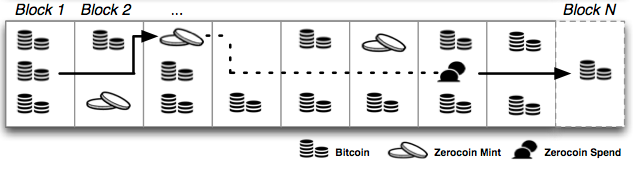
\includegraphics[width=0.7\textwidth]{zerocoin-chain.png}
\end{figure}

Монета Zerocoin \textbf{чеканится} путём сжигания известной монеты Bitcoin и добавления в накопитель монет. Zerocoin \textbf{тратится} путём доказательства владения неизвестной монетой в накопителе, которая переводится в Bitcoin.
\end{frame}


\begin{frame}{Пример: Zerocoin}
\begin{columns}
\begin{column}{0.7\textwidth}
Плюсы:
\begin{itemize}
\item накопители гарантируют максимальную неопределённость траты;
\item прекрасно работает с прозрачными активами.
\end{itemize}

Минусы:
\begin{itemize}
\item возможность того, что будут сожжены активы честных пользователей;
\item взломанное с целью повышения инфляции доказательство создания («чеканки») монеты;
\item ограничение до фиксированной суммы при отсутствии прямой передачи;
\item большие и неэффективные доказательства;
\item данные времени и связывания переносятся в основной блокчейн.
\end{itemize}
\end{column}
\begin{column}{0.3\textwidth}
\begin{figure}

\includegraphics[width=0.6\textwidth]{zerocoin.png}
\end{figure}
\end{column}
\end{columns}
\end{frame}


\begin{frame}{Zerocash/Zcash}
\textbf{Zerocash} был протоколом транзакций, повлиявшим на протоколы \textbf{Zcash}. Текущие протоколы используют накопители на основе дерева Меркла, но гораздо более гибко, чем Zerocoin, благодаря более устойчивым системам доказательства. \\~\\

Транзакции поддерживают прямую передачу скрытых сумм, скрывая траты внутри накопителей. Анонимность обеспечивается опционально.

\begin{figure}
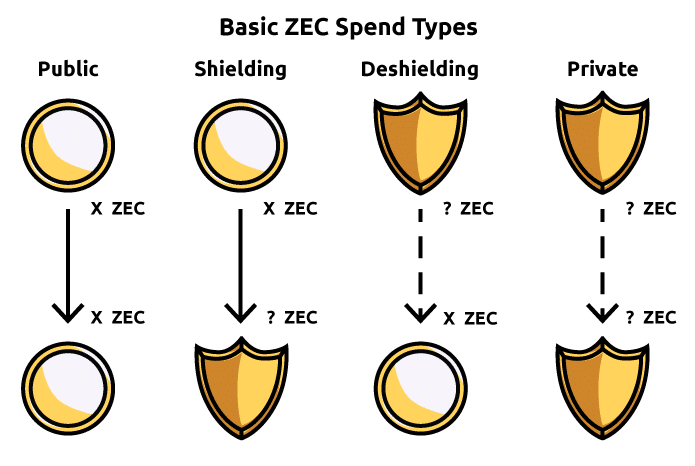
\includegraphics[width=0.4\textwidth]{zcash-types.png}
\end{figure}
\end{frame}


\begin{frame}{Пример: Zerocash/Zcash}
\begin{columns}
\begin{column}{0.7\textwidth}
Плюсы:
\begin{itemize}
\item накопители гарантируют максимальную неопределённость траты;
\item прекрасно работает с прозрачными активами;
\item поддерживает прямые передачи;
\item малый размер доказательства и эффективная верификация.
\end{itemize}

Минусы:
\begin{itemize}
\item целостность системы доказательства требует отсутствия конфликтов и правильности MPC;
\item сложность структуры из-за более общего характера системы доказательства;
\item опциональный характер анонимности;
\item транзакции допускают анализ связывания и времени.
\end{itemize}
\end{column}
\begin{column}{0.3\textwidth}
\begin{figure}

\includegraphics[width=0.6\textwidth]{zcash.png}
\end{figure}
\end{column}
\end{columns}
\end{frame}


\begin{frame}{Зачем так много подходов?}
\begin{itemize}
\item \textbf{Прозрачное смешивание}, по сути, не обеспечивает \textit{никакой} анонимности и даёт очень низкий уровень взаимозаменяемости, но позволяет сохранить совместимость с открытыми реестрами за счёт использования интерактивных процессов.
\item Подходы, предполагающие \textbf{сокрытие / неопределённость} могут обеспечить разумный уровень анонимности и взаимозаменяемости, но за счёт эффективности и возможности применения некоторых методов анализа графов.
\item \textbf{Общие системы доказательства} могут использоваться для построения небольших и быстрых транзакций в рамках моделей транзакций, основанных на использовании накопителей, с хорошим уровнем анонимности, но практически за счёт гарантий целостности. \\~\\
\end{itemize}
\end{frame}


\begin{frame}{Модель транзакции и система доказательства}
\textbf{Модель транзакции} является набором криптографических конструкций (подписей, доказательств), используемых для демонстрации таких вещей, как право владения активом, отсутствие двойной траты, баланс, место назначения и так далее. Нами были рассмотрены несколько.

\textbf{Система доказательства} является криптографической конструкцией, используемой для доказательства и верификации математически определяемых утверждений, включающих приватные и публичные данные, в идеале — с нулевым разглашением.

\begin{itemize}
\item Наличие системы доказательства не даёт нам модели транзакции. Наличие языка бесполезно, если вам нечего сказать.
\item Конструкции в некоторых моделях транзакций могут быть построены с использованием систем доказательства для создания и верификации транзакций, но тут мы сталкиваемся с рядом препятствий, связанных с эффективностью и специфичностью. Природа контрольной последовательности играет важную роль (например, в случае с ZCash и связанными с ней активами).
\end{itemize}
\end{frame}


\begin{frame}
\begin{figure}
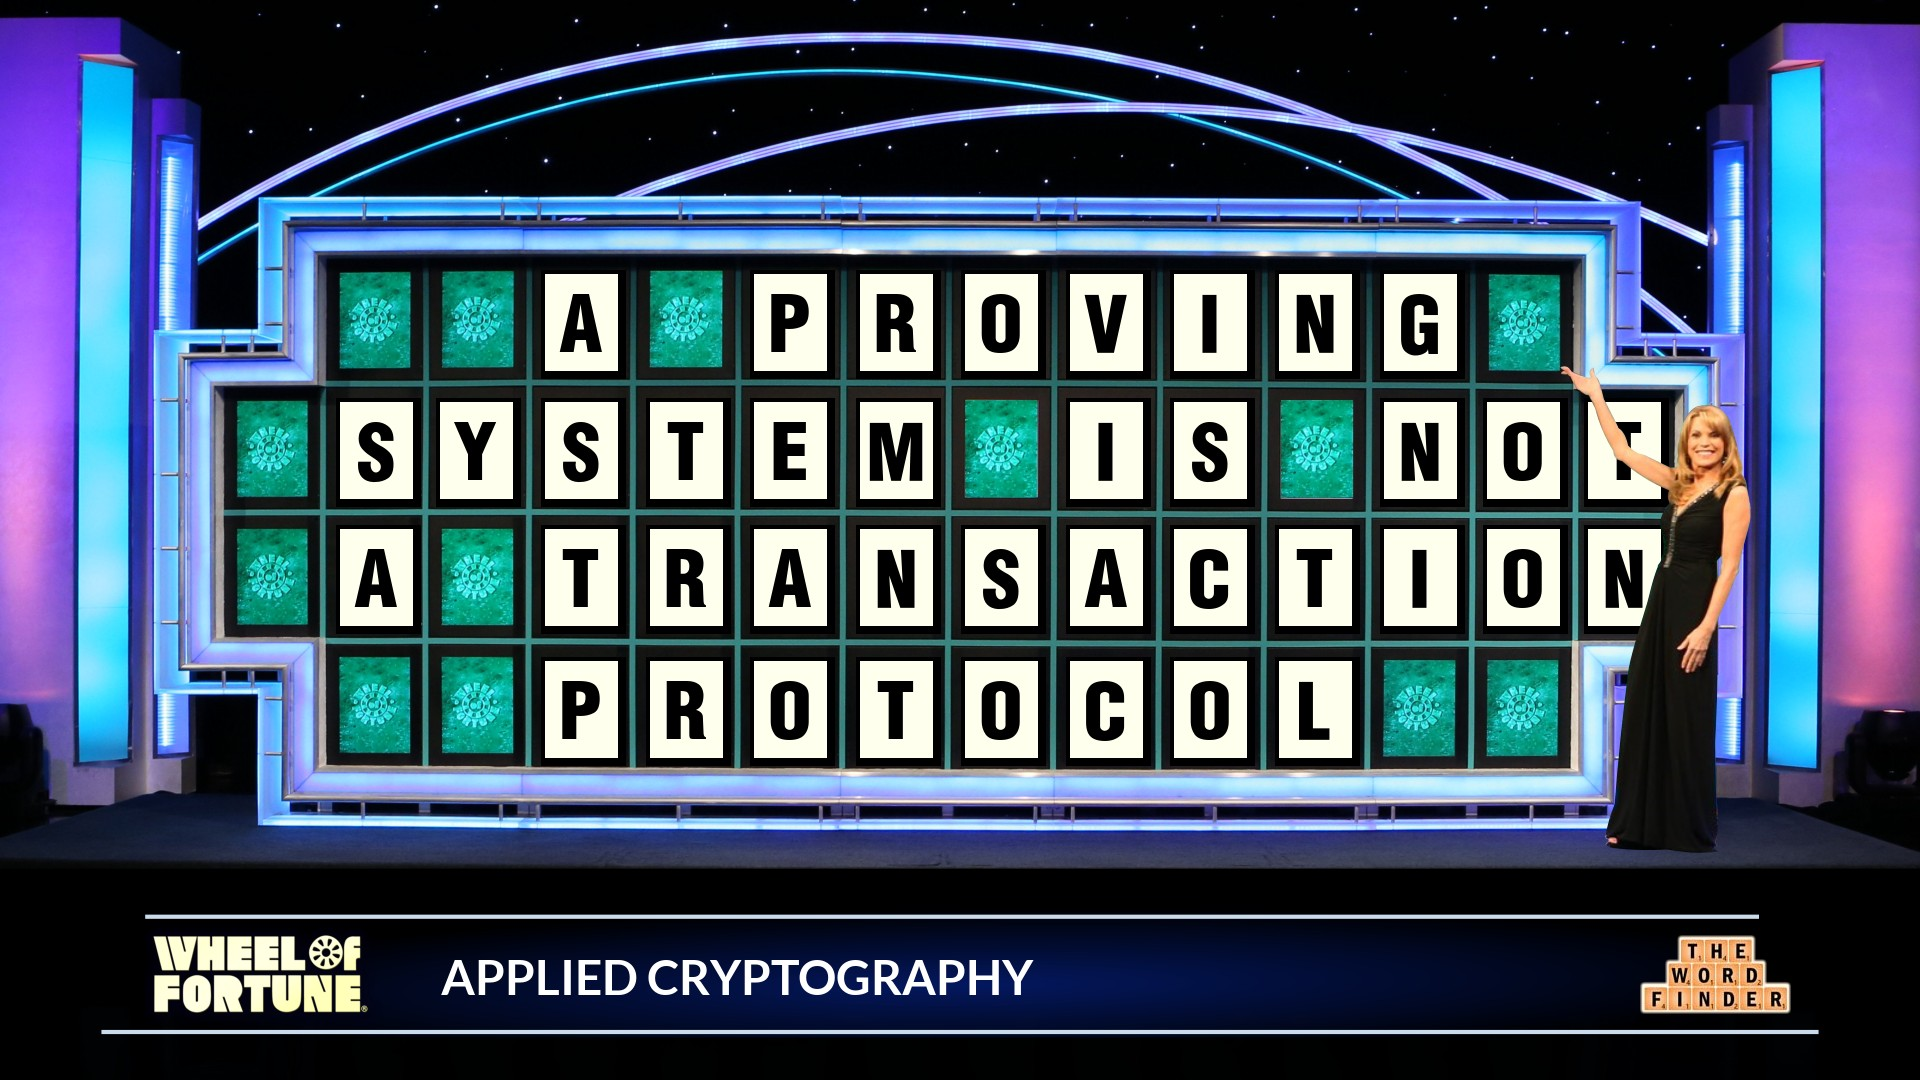
\includegraphics[width=\textwidth]{puzzle.jpeg}
\end{figure}
\end{frame}


\begin{frame}{Метаданные имеют значение}
\begin{table}
\centering
\begin{tabular}{>{\arraybackslash}m{0.3in} >{\arraybackslash}m{2.0in}}

\includegraphics[width=20px]{icon-earth.png} & Сетевые данные / данные местоположения \\

\includegraphics[width=20px]{icon-web.png} & Ретрансляция транзакций \\

\includegraphics[width=20px]{icon-arrows.png} & Структура ввода-вывода \\

\includegraphics[width=20px]{icon-stopwatch.png} & Временные данные / периодичность \\

\includegraphics[width=20px]{icon-clip.png} & Связывание адресов \\
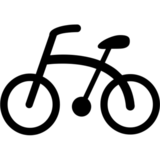
\includegraphics[width=20px]{icon-bike.png} & Перемещения / переводы \\

\includegraphics[width=20px]{icon-spy.png} & Атаки по сторонним каналам
\end{tabular}
\end{table}

\begin{center}
\textbf{Лучшие модели транзакции в мире не обеспечивают удаления всех метаданных!}
\end{center}
\end{frame}


\begin{frame}{Направления исследований}
\begin{figure}
\begin{tikzpicture}[thick]
\node (q) {\textbf{Готовы ли вы доверить обеспечение целостности третьим сторонам?}};
\node [circle,draw,below=50pt,left=100pt,at=(q.south),fill=green!30] (yes) {Да};
\node [circle,draw,below=50pt,right=100pt,at=(q.south),fill=red!30] (no) {Нет};

\draw [-] (q) -- (yes);
\draw [-] (q) -- (no);
\end{tikzpicture}
\end{figure}
\begin{columns}
\begin{column}{0.5\textwidth}
Существуют хорошие системы доказательства, на основе которых можно построить быстрые и эффективные протоколы транзакций, которые будут обеспечивать анонимность и конфиденциальность на основе использования накопителей.
\end{column}
\begin{column}{0.5\textwidth}
Опции по большей части имеют узкоспециальный характер и страдают от проблем с масштабированием подписей и размера доказательства. Процесс верификации обычно масштабируется так же плохо, как и размер.
\end{column}
\end{columns}
\end{frame}


\begin{frame}{Пример: MMORPG (Zcash Sapling)}
\textbf{MMORPG} вариант системы доказательства, предложенный Боуи \textit{и др.} от Groth. Он доказывает утверждения относительно соответствия схемы с нулевым разглашением. \\~\\

Требуются структурированные/доверенные настройки, но они являются распределёнными. Размер доказательства составляет менее 200 байт для схемы любой сложности. Доказательство является линейным для сложности схемы, но верификация будет линейной только для сложности свидетельства. \\~\\
\end{frame}
\begin{frame}
В случае со схемой ZCash Sapling время доказательства составляет $O(1)$ секунд, а время верификации - $O(1)$ миллисекунд. (Здесь время доказательства зависит от не общей оптимизации схем!) \\~\\

Используется:
\begin{figure}

\includegraphics[height=50pt]{zcash.png}
\end{figure}
\end{frame}


\begin{frame}{Пример: Bulletproofs}
\textbf{Bulletproofs} является расширением, предложенным Бюнцем \textit{и др.} для основной системы доказательств, авторами которой являются Бутль \textit{и др.} Расширение доказывает утверждения относительно соответствия схемы с нулевым разглашением. \\~\\

Структурированные или доверенные настройки отсутствуют; контрольные последовательности генерируются публично. Размер является логарифмическим (сублинейным) для сложности схемы, но доказательство и верификация происходят линейно. \\~\\
\end{frame}
\begin{frame}
Для \underline{оценки} схемы ZCash Sapling: время доказательства составляет $O(10)$ секунд, а время верификации - $O(1)$ секунд (и вплоть до $O(100)$ миллисекунд) при размере доказательства $O(1)$ Кбайт. \\~\\

Используется (только при оптимизированном доказательстве диапазона):
\begin{figure}

\includegraphics[align=c,height=42pt]{logo-beam.png}

\includegraphics[align=c,height=55pt]{logo-grin.png}

\includegraphics[align=c,height=50pt]{logo-monero.png}
\end{figure}
\end{frame}


\begin{frame}{Дикое упрощение}
\begin{table}
\centering
\begin{tabular}{>{\arraybackslash}m{1.0in} >{\arraybackslash}m{0.5in} >{\arraybackslash}m{0.5in} >{\arraybackslash}m{1.0in}}
& Боуи\footnote{IACR 2017/1050} & Бюнц\footnote{IACR 2017/1066} & Бен-Сассон\footnote{IACR 2018/046} \\
\hline
Отсутствие доверенных настроек & \nicon & \yicon & \yicon \\
Размер доказательства & \yicon & \yicon & \nicon \\
Скорость доказательства* & \nicon & \nicon & \nicon \\
Скорость верификации & \yicon & \nicon & \yicon
\end{tabular}
\end{table}
\begin{center}
* крайне зависит от варианта реализации и схемы
\end{center}
\end{frame}


\begin{frame}{Цель}
Целью современных исследований является выработка \textbf{общих систем доказательства, не требующих доверенных настроек} для обеспечения целостности и практической эффективности. \\~\\

В одной интересной работе было предложено использовать универсальную и/или обновляемую контрольную последовательность, но и тут есть некоторая возможность использования доверенной модели. \\~\\

\begin{center}
\textbf{Всё гораздо замысловатее, чем звучит, даже если это уже звучит замысловато.}
\end{center}
\end{frame}


\begin{frame}{Спасибо}
\textbf{Рад ответить на ваши вопросы.} \\~\\

Анонимность транзакций и взаимозаменяемость активов - сложная и нерешённая проблема, поэтому, пожалуйста, задавайте вопросы. \\~\\

\begin{center}
\Large \texttt{sarang.noether@protonmail.com}
\end{center}
\end{frame}

\end{document}